\documentclass{article}


\usepackage{arxiv}

\usepackage[utf8]{inputenc} % allow utf-8 input
\usepackage[T1]{fontenc}    % use 8-bit T1 fonts
\usepackage{hyperref}       % hyperlinks
\usepackage{url}            % simple URL typesetting
\usepackage{booktabs}       % professional-quality tables
\usepackage{amsfonts}       % blackboard math symbols
\usepackage{nicefrac}       % compact symbols for 1/2, etc.
\usepackage{microtype}      % microtypography
\usepackage{lipsum}
\usepackage{graphicx}
\usepackage{float}
\graphicspath{ {./img/} }

\title{Unsupervised MRI brain image segmentation}

\author{
  Sarah Xu \\
  \texttt{sarahxu@stanford.edu} \\
  %% examples of more authors
   \And
 Yuxin Hu \\
  \texttt{yuxinh@stanford.edu} \\
  \And
 Zhaotian Fang \\
  \texttt{z23fang@stanford.edu} \\
  %% \AND
  %% Coauthor \\
  %% Affiliation \\
  %% Address \\
  %% \texttt{email} \\
  %% \And
  %% Coauthor \\
  %% Affiliation \\
  %% Address \\
  %% \texttt{email} \\
  %% \And
  %% Coauthor \\
  %% Affiliation \\
  %% Address \\
  %% \texttt{email} \\
}

\begin{document}
\maketitle
% keywords can be removed
\keywords{tumor segmentation \and neuroanatomy segmentation \and super-resolution \and medical imaging \and unsupervised learning }

\section{Introduction}
In recent years, there has been renewed interest in accurate segmentation of magnetic resonance (MR) images, especially for the human brain. In this task, there are two focus areas: neuroanatomy segmentation on the whole brain as well as anomaly detection and segmentation on the lesion or tumor areas. 

Since manual segmentation of brain neuroanatomy and lesions is time-consuming, there has been a plethora of efforts in automating and accelerating the process. For brain neuroanatomy segmentation, the most commonly used is a software tool named FreeSurfer.~\cite{freesurfer} However, this tool is computationally intensive, taking several hours for one person. As for brain lesion segmentation, radiologists use a MATLAB toolbox named Lesion Segmentation Tool (LST) to gather initial results, and then manually adjust the detected regions.~\cite{schmidt2013lst}

In attempt to improve on the efficiency and accuracy of the segmentation, supervised deep learning methods have been emerging over the past few years.~\cite{badrinarayanan2017segnet, su2015autoencoder, li2018hdensenet, wachinger2018deepnat} However, there are two main shortcomings to these methods. First, these supervised methods require an extensive amount of high-quality segmentation labels, which made by radiologists and thus hard to obtain. Secondly, supervised approaches struggle with generalization across different datasets. In the context of brain MRIs, the image distribution varies drastically based on the process used to obtain them (e.g. the machine). Therefore, a model trained on one dataset may not perform as well on other datasets. Therefore, there is a need to find a dataset-agnostic model to effectively segment the brain MR images in an unsupervised manner.

There have been a few efforts in applying unsupervised and semi-supervised methods for brain MRI segmentation. Stacked denoising autoencoders were used as a pre-training step before supervised learning.~\cite{su2015autoencoder} Generative models such as the AnoGAN framework and Variational Autoencoders were trained purely on healthy brain images, assuming that the network would be able to detect the abnormal regions.~\cite{an2015vae, Januszewsk2019cyclegan} However, those methods still need large sets of healthy images, and can only be used for rough tumor segmentation, since some high-resolution details are missed. In this work, we want to simultaneously segment brain anatomy and lesions without the need of labelling.

Another branch of methods used in improving segmentation is through super-resolution. Since high-resolution brain MR images are scarce, efforts have been made to build a model that upsamples low-resolution images so it can then be segmented to produce a finer result. We also want to explore the idea of learning these tasks jointly using deep learning. Research into this joint task is limited. Pham et. al showed that their model SegSRGAN, a WGAN that learns both tasks jointly, was able to outperform state-of-the-art models trained on individual tasks.~\cite{pham:hal-01895163} Sun et. al proposed a supervised U-Net based model that learns both image reconstruction and segmentation of brain CS-MRIs.~\cite{sun2018joint}

%An effort was made to combine the above-mentioned frameworks into what is called AnoVAEGAN to segment brain lesions in an unsupervised way. However, these approaches are still rely on large sets of high-quality and healthy brain images to learn effectively.

\section{Method}
% Define the input-output behavior of the system and the scope of the project.
Mutual information measures the mutual dependence between the two variables, and it has been used for image registration, feature selection, etc. Recently, a method called invariant information clustering (IIC) was proposed and achieved state-of-the-art results for unsupervised image classification and segmentation.~\cite{ji2018invariant} This method maximizes the mutual information between the class assignments of each pair and can directly output labelling on each pixel. In this project, we plan to use a similar idea to segment both neuroanatomy and lesion in an unsupervised manner. The inputs to our system are unlabeled brain MR images. The output to our system consists of segmentation masks with labels for different anatomical components and lesions.

\subsection{Challenges}
% What are the challenges? Which topics (e.g., search, MDPs, etc.) might be able to address those challenges (at a high-level, since we haven't covered any techniques in detail at this point)?
% challenges be what is difficult about solving this problem without the use of AI, or should it be more about what problems might arise when trying to implement our methods?
Accurate image segmentation itself is very challenging, even with labels. This is especially the case for medical images, considering the variance in images produced by different patients, hardware, and radiologists. Traditional image segmentation comprise of various edge-based and region-based methods.\cite{segmentation_survey} However, these methods are not robust and do not generalize well across different datasets. Supervised learning methods using deep neural networks have shown to achieve state-of-the-art results given a sufficient amount of training examples. 

During the implementation of our system, we may observe that IIC will not be able to learn the best segmentation from brain MRIs. Although IIC has been shown to work with image distributions occurring in nature, it is unclear how well the method will transfer to MR images. Another challenge we face is proper evaluation of segmentation results. More specifically, there is no standard metric for brain anatomy segmentation. In addition, it is hard to tell the extent of tumors in MR images, even for trained professionals like radiologists.

\subsection{Dataset}
% Collect some preliminary data, and give concrete examples of inputs and outputs.
Our data will mainly come from two sources. The first source is the Human Connectome Project (HCP), which provides MR images of $1206$ healthy young adults subjects collected in 2012 to 2015, where 3T structural scans are available for 1113 subjects.~\cite{van2012human} Additional brain lesion data are available from the 2008 Medical Image Computing and Computer Assisted Intervention (MICCAI) multiple sclerosis (MS) Lesion Segmentation Challenge where 54 brain MR images and represents a range of patients and pathology which was acquired from Children's Hospital Boston and University of North Carolina.~\cite{miccai2008}

We may also be able to test our trained network on some clinical data from our collaborators at Massachusetts General Hospital (MGH) and Stanford hospital.

\subsection{Baseline and Oracle}
\paragraph{Baseline}
For the baseline of the project, the anatomy segmentation is obtained using a unsupervised segmentation method called mean-shift clustering. This method perform iterative mean-shift algorithm at each pixel until they converge to a set of clusters. ~\cite{comaniciu1999mean} For the example shown in Fig. 1b, the brain image is segmented into 17 clusters.

For the tumor segmentation, we use LST with lesion prediction algorithm (LPA) on Fluid-attenuated inversion recovery (FLAIR) MR images to obtain a baseline for the lesion segmentation (Fig. 2b).~\cite{ediss20373}

\paragraph{Oracle}
As shown in Fig. 1c, We will be using the FreeSurfer segmentation results as the oracle for neuroanatomy segmentation on MR images, which classify the brain regions into labels ranging from $0$ to $14175$.~\cite{freesurfercolorlut}  Radiologist's manual labelling of brain lesion is used as the oracle for lesion segmentation.

\subsection{Evaluation}
% What is your evaluation metric for success?
To evaluate the quality of the segmentation results, we can employ three metrics commonly used for this task. Long et. al introduced pixel accuracy and mean intersection over union (mIOU) as metrics in evaluating their FCN for semantic segmentation. Another common segmentation metric used in the medical imaging field is the DICE coefficient.~\cite{dice1945measures} Brebisson et. al used the mean DICE coefficient over classes to evaluate their novel CNN for anatomical brain segmentation.

Observer study is another way to get signal on the performance of the model. More specifically, we will hand pairs of ground truth and predicted segmentation results to radiologists for them to score the quality.

\newpage
\begin{figure}[H]
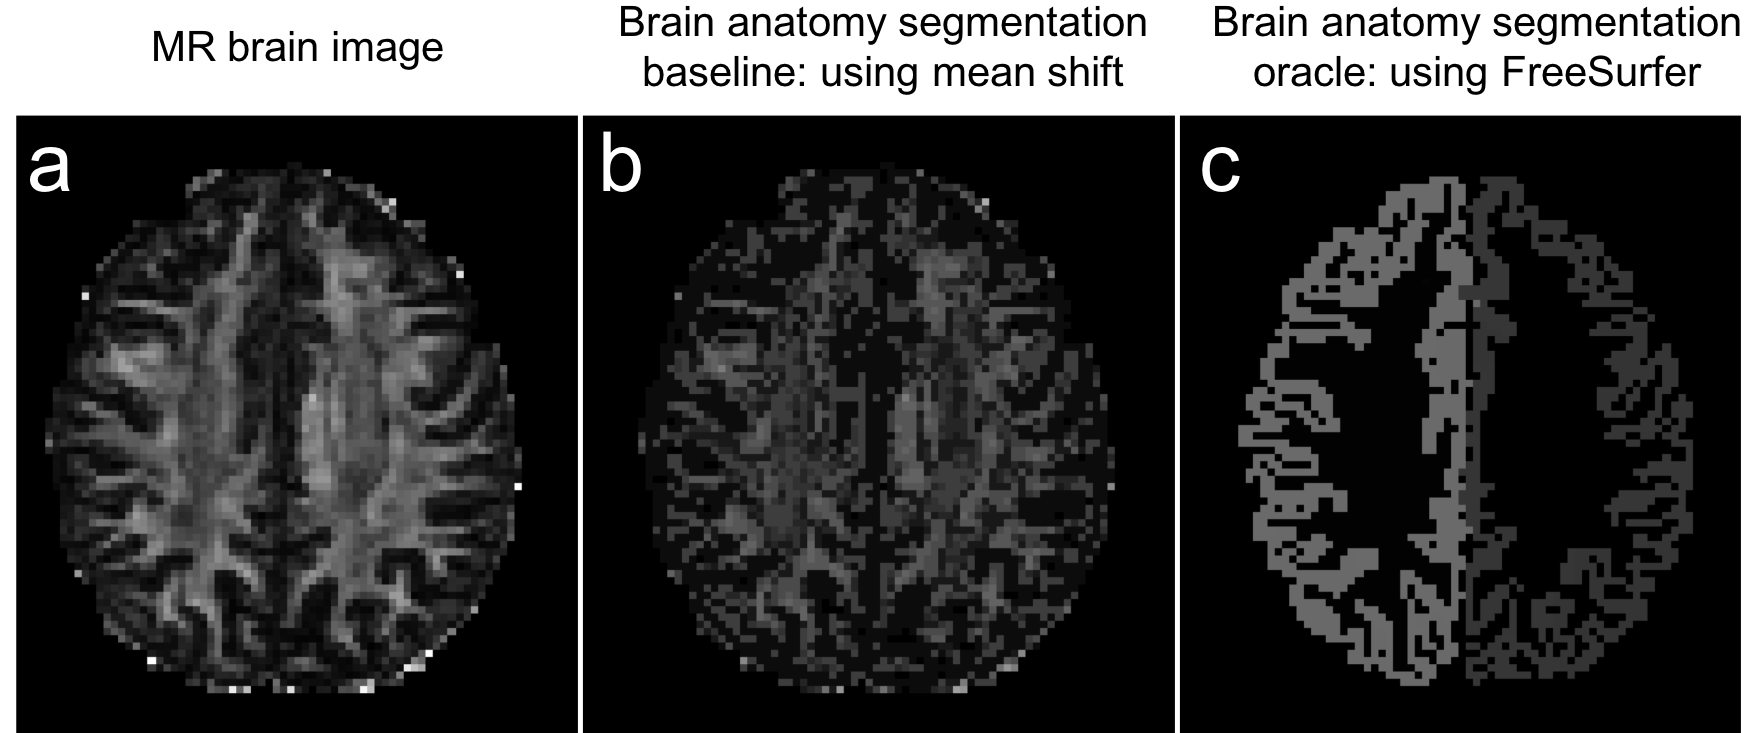
\includegraphics[width=\textwidth]{img/Picture1.png}
\caption{Example anatomy segmentation of brain MRI with mean shift (baseline) and FreeSurfer (orcale).}
\label{fig1:anatomy}
\end{figure}

\begin{figure}[H]
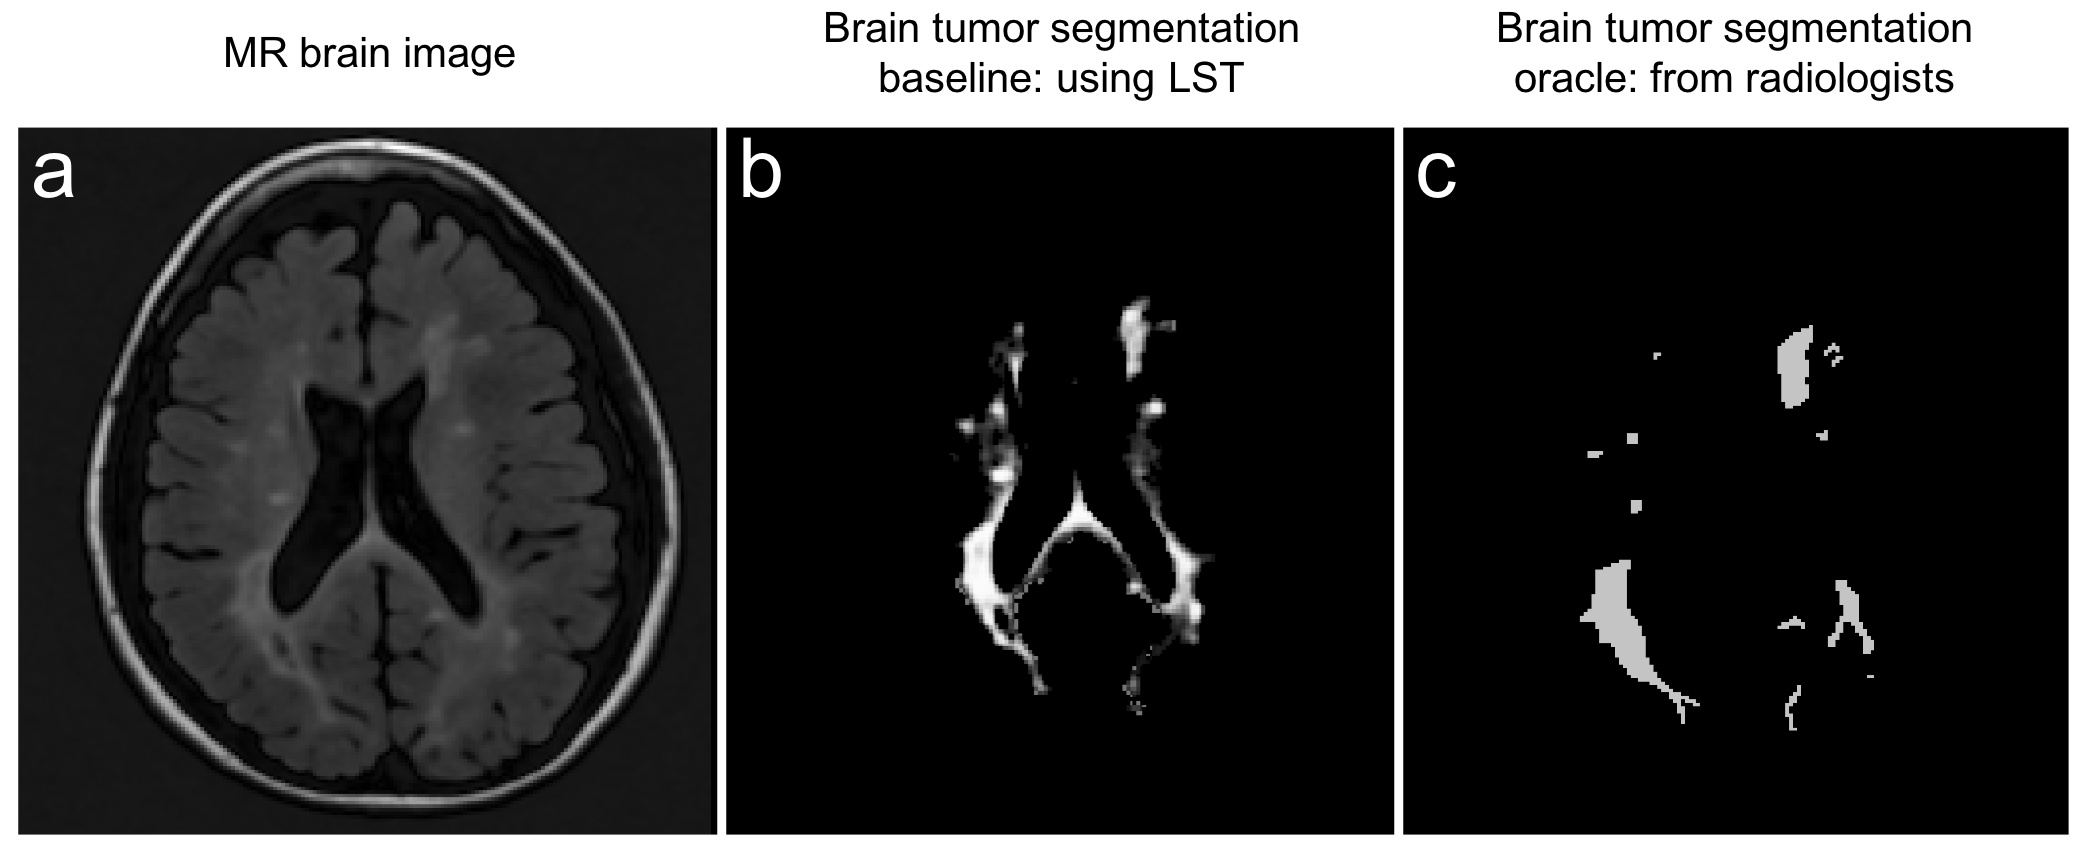
\includegraphics[width=\textwidth]{img/Picture2.png}
\caption{Example tumor segmentation of brain MRI with LST package (baseline) and radiologist's manual drawing (orcale).}
\label{fig2:tumor}
\end{figure}


\bibliographystyle{unsrt}  
\bibliography{proposal}  %%% Remove comment to use the external .bib file (using bibtex)

\end{document}
